
%(BEGIN_QUESTION)
% Copyright 2010, Tony R. Kuphaldt, released under the Creative Commons Attribution License (v 1.0)
% This means you may do almost anything with this work of mine, so long as you give me proper credit

Anta at lampen nekter å lyse når trykknappbryteren trykkes inn. Et voltmeter viser 0 volt mellom testpunktene {\bf A} og {\bf D} i kretsen mens trykknappen holdes inne:

$$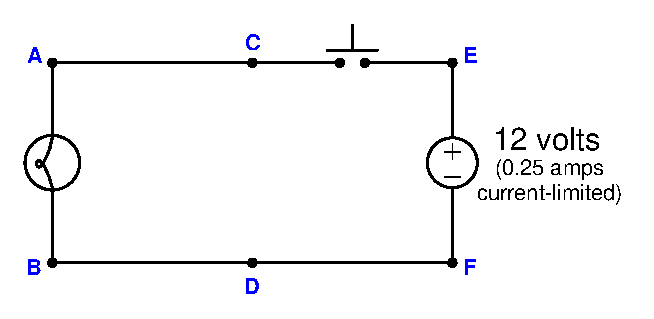
\includegraphics[width=15.5cm]{i01555x01.eps}$$

Bestem diagnostisk verdi av hver av følgende tester. Anta bare én feil i systemet, inkludert en enkelt komponent eller en enkelt ledning/kabel/rørforbindelse mellom komponenter. Hvis en foreslått test kan gi ny informasjon som hjelper deg å identifisere plassering og/eller type feil, marker ``ja''. Hvis en foreslått test ikke vil gi noe relevant for å identifisere feilen (allerede utledbart fra målinger og symptomer så langt), marker ``nei''.

% No blank lines allowed between lines of an \halign structure!
% I use comments (%) instead, so that TeX doesn't choke.

$$\vbox{\offinterlineskip
\halign{\strut
\vrule \quad\hfil # \ \hfil & 
\vrule \quad\hfil # \ \hfil & 
\vrule \quad\hfil # \ \hfil \vrule \cr
\noalign{\hrule}
%
% First row
{\bf Diagnostisk test} & {\bf Ja} & {\bf Nei} \cr
%
\noalign{\hrule}
%
% Another row
Mål $V_{EF}$ med bryteren inntrykket &  &  \cr
%
\noalign{\hrule}
%
% Another row
Mål $V_{CD}$ med bryteren inntrykket &  &  \cr
%
\noalign{\hrule}
%
% Another row
Mål $V_{CB}$ med bryteren inntrykket &  &  \cr
%
\noalign{\hrule}
%
% Another row
Mål $V_{CE}$ med bryteren inntrykket &  &  \cr
%
\noalign{\hrule}
%
% Another row
Mål $R_{AB}$ med bryteren inntrykket &  &  \cr
%
\noalign{\hrule}
%
% Another row
Mål $V_{EF}$ med bryteren ikke inntrykket &  &  \cr
%
\noalign{\hrule}
%
% Another row
Mål $V_{CD}$ med bryteren ikke inntrykket &  &  \cr
%
\noalign{\hrule}
%
% Another row
Mål $V_{CB}$ med bryteren ikke inntrykket &  &  \cr
%
\noalign{\hrule}
%
% Another row
Mål $V_{CE}$ med bryteren ikke inntrykket &  &  \cr
%
\noalign{\hrule}
%
% Another row
Mål $R_{AB}$ med bryteren ikke inntrykket &  &  \cr
%
\noalign{\hrule}
} % End of \halign 
}$$ % End of \vbox

\vfil 

\underbar{file i01555}
\eject
%(END_QUESTION)





%(BEGIN_ANSWER)

% No blank lines allowed between lines of an \halign structure!
% I use comments (%) instead, so that TeX doesn't choke.

$$\vbox{\offinterlineskip
\halign{\strut
\vrule \quad\hfil # \ \hfil & 
\vrule \quad\hfil # \ \hfil & 
\vrule \quad\hfil # \ \hfil \vrule \cr
\noalign{\hrule}
%
% First row
{\bf Diagnostisk test} & {\bf Ja} & {\bf Nei} \cr
%
\noalign{\hrule}
%
% Another row
Mål $V_{EF}$ med bryteren inntrykket & $\surd$ &  \cr
%
\noalign{\hrule}
%
% Another row
Mål $V_{CD}$ med bryteren inntrykket & $\surd$ &  \cr
%
\noalign{\hrule}
%
% Another row
Mål $V_{CB}$ med bryteren inntrykket & $\surd$ &  \cr
%
\noalign{\hrule}
%
% Another row
Mål $V_{CE}$ med bryteren inntrykket & $\surd$ &  \cr
%
\noalign{\hrule}
%
% Another row
Mål $R_{AB}$ med bryteren inntrykket & $\surd$ &  \cr
%
\noalign{\hrule}
%
% Another row
Mål $V_{EF}$ med bryteren ikke inntrykket & $\surd$ &  \cr
%
\noalign{\hrule}
%
% Another row
Mål $V_{CD}$ med bryteren ikke inntrykket &  & $\surd$ \cr
%
\noalign{\hrule}
%
% Another row
Mål $V_{CB}$ med bryteren ikke inntrykket &  & $\surd$ \cr
%
\noalign{\hrule}
%
% Another row
Mål $V_{CE}$ med bryteren ikke inntrykket & $\surd$ &  \cr
%
\noalign{\hrule}
%
% Another row
Mål $R_{AB}$ med bryteren ikke inntrykket & $\surd$ &  \cr
%
\noalign{\hrule}
} % End of \halign 
}$$ % End of \vbox

%(END_ANSWER)





%(BEGIN_NOTES)


%INDEX% Troubleshooting review: electric circuit diagnostic test usefulness

%(END_NOTES)

